\documentclass{beamer}

\mode<presentation> {

%\usetheme{default}
%\usetheme{AnnArbor}
%\usetheme{Antibes}
%\usetheme{Bergen}
%\usetheme{Berkeley}
%\usetheme{Berlin}
%\usetheme{Boadilla}
%\usetheme{CambridgeUS}
%\usetheme{Copenhagen}
%\usetheme{Darmstadt}
%\usetheme{Dresden}
%\usetheme{Frankfurt}
%\usetheme{Goettingen}
%\usetheme{Hannover}
%\usetheme{Ilmenau}
%\usetheme{JuanLesPins}
%\usetheme{Luebeck}
%\usetheme{Madrid}
%\usetheme{Malmoe}
%\usetheme{Marburg}
%\usetheme{Montpellier}
%\usetheme{PaloAlto}
%\usetheme{Pittsburgh}
%\usetheme{Rochester}
%\usetheme{Singapore}
%\usetheme{Szeged}
%\usetheme{Warsaw}
\usetheme{Aalto}

%\usecolortheme{albatross}
%\usecolortheme{beaver}
%\usecolortheme{beetle}
%\usecolortheme{crane}
%\usecolortheme{dolphin}
%\usecolortheme{dove}
%\usecolortheme{fly}
%\usecolortheme{lily}
%\usecolortheme{orchid}
%\usecolortheme{rose}
%\usecolortheme{seagull}
%\usecolortheme{seahorse}
%\usecolortheme{whale}
%\usecolortheme{wolverine}

%\setbeamertemplate{footline}
%\setbeamertemplate{footline}[page number]

%\setbeamertemplate{navigation symbols}{}
}

\usepackage{graphicx}
\usepackage{booktabs}
\usepackage{amsmath}

\title{ELFI: Engine for Likelihood Free Inference}

\author{Antti Kangasr\"a\"asi\"o}
\institute[Probabilistic Machine Learning Group]
{
Aalto University, Probabilistic Machine Learning Research Group\\
\medskip
Joint work with:
Jarno Lintusaari (Aalto),
Henri Vuollekoski (Aalto),
Kusti Skyt\'en (Aalto),
Marko J\"arvenp\"a\"a (Aalto),
Michael Gutmann (University of Edinburgh),\\
Aki Vehtari (Aalto),
Jukka Corander (University of Oslo),
Samuel Kaski (Aalto)\\
\medskip
European Meeting of Statisticians 2017 Helsinki\\
\medskip
Slides and the demo are available at: \url{github.com/elfi-dev/zoo} (branch \textbf{ems2017})
}
\date{July 25th, 2017}

\begin{document}

\begin{frame}
\titlepage
\end{frame}

\begin{frame}
\frametitle{Overview}
\tableofcontents
\end{frame}

%------------------------------------------------
\section{Approximate Bayesian Computation}
%------------------------------------------------

\subsection{What is ABC}

\begin{frame}
\frametitle{Likelihood function}
Likelihood function is central in model-based inference\\
\medskip
In many cases, inference might consist of just finding the maximum of the likelihood function (ML point estimate)\\
\medskip\pause
However, with many complex models either:
\begin{itemize}
\item No explicit likelihood function exists
\item Evaluating the likelihood function is very expensive
\end{itemize}
\medskip\pause
Examples include:
\begin{itemize}
\item Climate models
\item Biological models
\item Cognitive models
\end{itemize}
\end{frame}

\begin{frame}
\frametitle{What is Approximate Bayesian Computation}
ABC is a set of inference methods that bypass the evaluation of the likelihood function\\
\medskip
The core idea in ABC is to repeatedly simulate predictions from the model and evaluate their discrepancy with the observation data\\
\medskip\pause
\textbf{Intuition:} If parameters lead to predictions that match with the observation data, then these parameters have high likelihood\\
\medskip\pause
ABC methods are based on Bayesian statistics, and with some assumptions we can closely approximate the true likelihood
\end{frame}

\begin{frame}
\frametitle{ABC Math Background}
Bayes' Rule says: $P(\theta | D) \propto P(D|\theta)P(\theta)$\\
\medskip
Thus, we can always estimate $P(\theta|D)$ with the rejection scheme:\\
\begin{itemize}
\item Draw $\theta \sim P(\theta)$ and $D \sim P(D|\theta)$
\item If $D = D_{obs}$, accept $\theta$ as a sample from $P(\theta | D_{obs})$
\end{itemize}
\medskip\pause
\textbf{Problem:} Is most cases our acceptance rate is nearly 0 as we require that $D = D_{obs}$ precisely\\
\medskip\pause
\textbf{Approx:} Accept samples when discrepancy $\delta(D, D_{obs}) < \varepsilon$, thus yielding samples from $P(\theta | \delta(D, D_{obs}) < \varepsilon)$\\
\medskip\pause
In general, this approach makes sense when evaluating the generative model is easier than evaluating the likelihood
\end{frame}

\subsection{Visual Demonstrations}

\begin{frame}
\frametitle{ABC Visual Demonstration 1}
\vspace{-1em}
\begin{figure}[ht]
\centerline{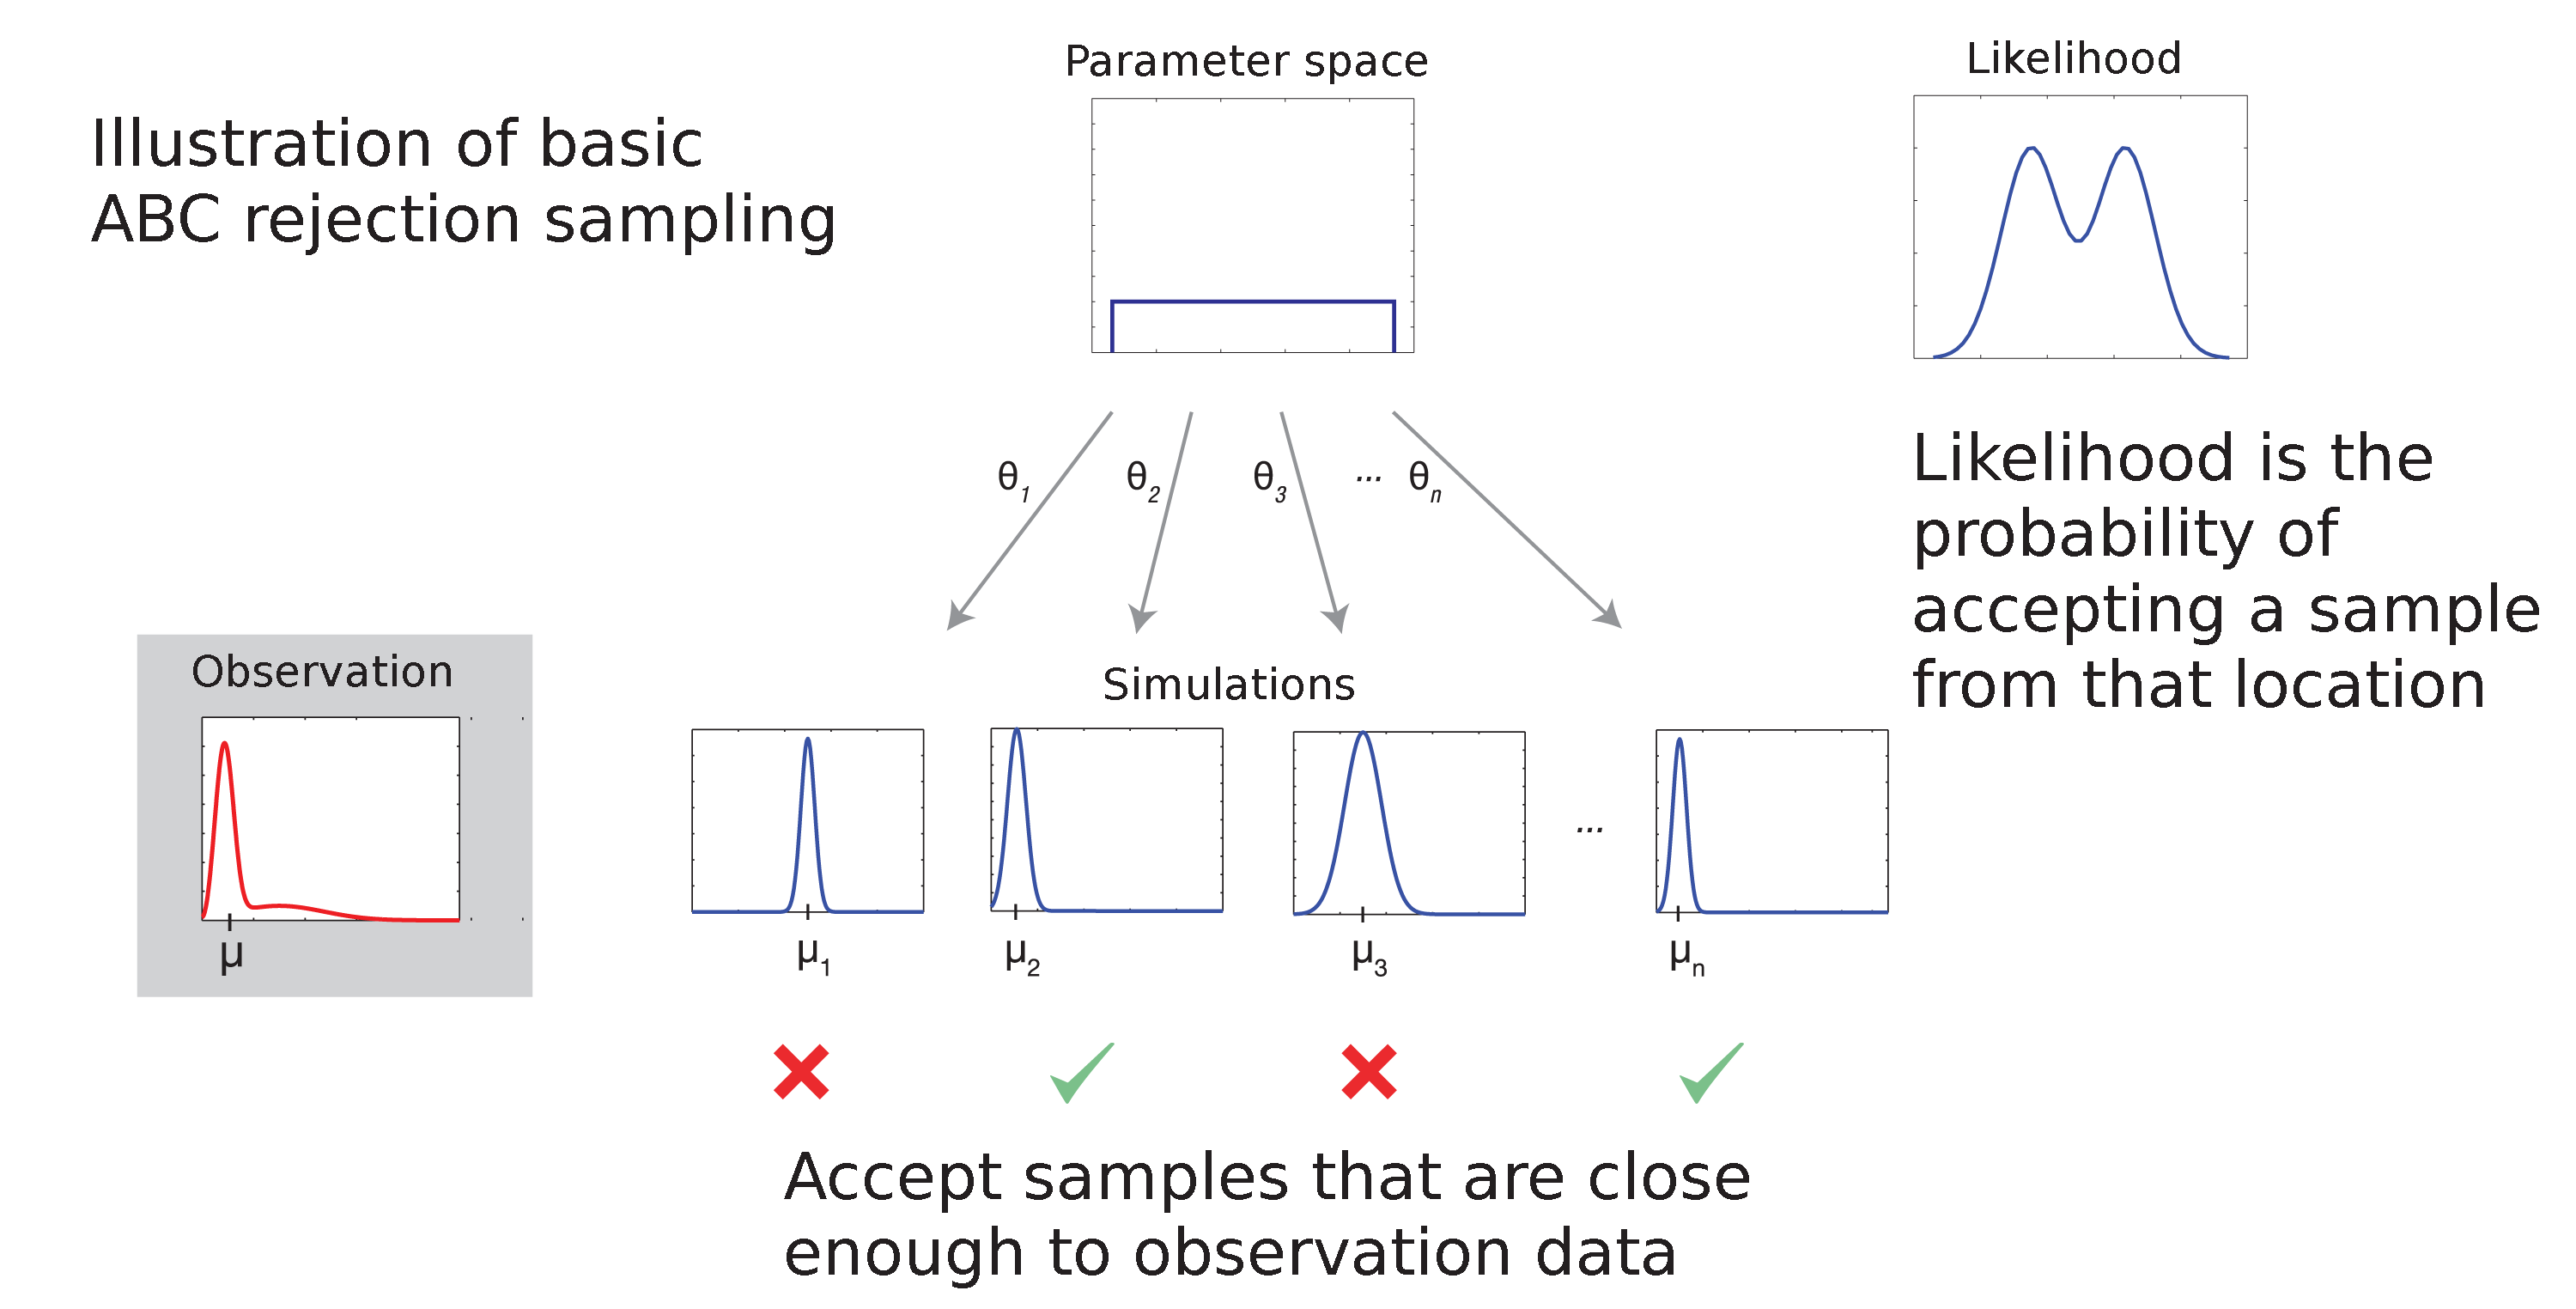
\includegraphics[width=\columnwidth]{img/abc1.png}}
\end{figure}
\vspace{-1em}
\tiny{Figure adapted from: Sunn{\aa}ker et al., 2013, \url{https://doi.org/10.1371/journal.pcbi.1002803}}
\end{frame}

\begin{frame}
\frametitle{ABC Design Parameters}
What one needs to choose to use ABC:
\begin{itemize}
\item Discrepancy function: $\delta(D_{sim}, D_{obs}) \rightarrow [0, \infty)$
\item Discrepancy threshold: $\varepsilon \in [0, \infty)$
\end{itemize}
\medskip
Choosing the discrepancy function is analogous to choosing a loss function: no perfect choice but some are more justified than others\\
\medskip
Threshold can even be chosen post-sampling if all samples can be stored in memory
\end{frame}

\newcommand{\filmslide}[1]{
\begin{frame}
 \frametitle{ABC Visual Demonstration 2}
 \begin{figure}[ht]
 \begin{center}
 \includegraphics[width=\textwidth]{./film/#1.png}
 \end{center}
 \end{figure}
 \bigskip
 \tiny{From (slides): Kangasr\"a\"asi\"o et al., 2017, \url{http://dl.acm.org/citation.cfm?id=3025576}}\\
 \tiny{Algorithm (BOLFI): Gutmann \& Corander, 2016, \url{http://jmlr.org/papers/v17/15-017.html}}
\end{frame}
}

\filmslide{01}
\filmslide{02}
\filmslide{03}
\filmslide{04}
\filmslide{05}
\filmslide{06}
\filmslide{07}
\filmslide{08}
\filmslide{09}
\filmslide{10}
\filmslide{11}
\filmslide{12}
\filmslide{13}
\filmslide{14}
\filmslide{15}
\filmslide{16}
\filmslide{17}
\filmslide{18}
\filmslide{19}
\filmslide{20}
\filmslide{21}
\filmslide{22}

%------------------------------------------------
\section{ELFI Python Library}
%------------------------------------------------

\subsection{What is ELFI}

\begin{frame}
\frametitle{Engine for Likelihood Free Inference}
ELFI is an open-source Python library that aims to make it easy for \textbf{practicioners} to apply ABC\\
\medskip
Main features of the library:
\begin{itemize}
\item Implementations of ABC algorithms
\item Easy syntax for defining model structure
\item Storage and re-use of results
\item Reporting and diagnostics tools
\end{itemize}
\end{frame}

\begin{frame}
\frametitle{ELFI for Developers}
ELFI aims to also become a platform where implementations of new methods can be easily published\\
\medskip
For \textbf{developers} ELFI offers:
\begin{itemize}
\item Modular design of the library
\item Well-defined API for implementing own modules
\item Development and maintenance of the library (by Aalto PML)
\item Growing user community
\end{itemize}
\end{frame}

\subsection{Demonstration}

\begin{frame}
\frametitle{Demonstration}
Live demonstration of the main features of ELFI\\
\medskip
Slides and the demo are available at:\\
\url{github.com/elfi-dev/zoo} (branch \textbf{ems2017})
\end{frame}

\end{document}
